\section{Formações}\label{sec:formacoes}

    Neste capítulo será feita uma análise breve de cada uma das tecnologias ou temas abordados durante as formações recebidas no início do estágio. Cada secção a seguir abordará uma tecnologia específica dada numa formação, apresentando uma visão geral, as principais características, a importância e o impacto que cada uma delas pode ter para o desenvolvimento profissional dos profissionais em contexto empresarial.

    Existe um caminho formativo bem definido para os novos contratados, comunicado através do DDC Academy (Deloitte Delivery Center) e do CURA, uma plataforma interna de formações onde nos foram passadas grande parte dos materiais e formações.

    Enquanto muitas das formações focam no aspeto prático das tecnologias, este capítulo será aproveitado para aprofundá-las e expor quaisquer mais informações relevantes.

    O estagiário começou o estágio um pouco depois da data inicialmente acordada por pedido, pelo que algumas das formações e atividades que os restantes recém-contratados comparticiparam na primeira metade do mês de setembro não foram aproveitadas pelo estagiário, na Figura \ref{fig:tempoform} no Anexo \ref{anexo_formacoes} está representado, através de um mapa de Gantt, o tempo dedicado a cada formação no período inicial do estágio, a primeira barra, começa antes do gráfico em si, pois esta formação estava já em decurso antes do começo do estágio, pelo que apenas parte da formação pode ser aproveitada.

    \subsection{Formação de PL/SQL}\label{subsec:pl-sql}

      \textit{Procedural Language/Structured Query Language}, mais conhecido por PL/SQL, é uma linguagem de programação criada pela Oracle para gestão das bases de dados Oracle. Foi criada de forma a integrar declarações SQL na sua sintaxe. Durante a execução, o PL/SQL e o SQL correm no mesmo processo do servidor, otimizando a sua eficiência\cite{what-is-pl/sql}.

      O PL/SQL combina a flexibilidade da programação procedimental com a capacidade de consulta de dados de SQL, possibilitando a utilização de uma panóplia de conceitos típicos de programação diretamente com SQL, como por exemplo:
      \begin{itemize}
          \item \textbf{\textit{Triggers} de Base de Dados:} Ações ou procedimentos automáticos desencadeados por eventos específicos ou alterações de dados na base de dados;
          
          \item \textbf{Funções:} O PL/SQL suporta a criação de funções, permitindo menos repetição e mais flexibilidade na organização de dados e código;
          
          \item \textbf{\textit{Procedures \& Function Overloading}:} Suporta o conceito de criar múltiplas versões de procedimentos ou funções com o mesmo nome, mas diferentes parâmetros, permitindo flexibilidade e reutilização de código;

          \item \textbf{Exceções}: Como muitas linguagens procedimentais, suporta também o lançamento e tratamento de exceções.
      \end{itemize}
      
      Em suma, o PL/SQL é uma extensão às bases de dados Oracle SQL, e facilita a interação com estas através de uma sintaxe mais familiar para quem está familiarizado com programação procedimental, oferecendo ao mesmo tempo, compatibilidade com a sintaxe do SQL\cite{sql-language-reference}.

    \subsection{Formação de Java}\label{subsec:java}

      Java é uma linguagem de programação amplamente utilizada no desenvolvimento de aplicações empresariais, aplicações móveis, sistemas integrados e muito mais. A sua portabilidade, orientação a objetos e robustez fazem dela uma escolha popular para uma variedade de aplicações.

      Foram exploradas as maneiras de planeamento de código mais usadas na indústria como o diagrama de casos de uso como o visto na Figura \ref{fig:vending_machine}, este diagrama identifica as diferentes interações entre atores externos e o sistema, destacando os principais casos de uso e as suas relações. Ajuda a visualizar as funcionalidades que o sistema oferece do ponto de vista do utilizador e fornece uma visão geral da interação entre os atores e os casos de uso.
      
      % scale svg in latex: https://tex.stackexchange.com/questions/390804/how-to-scale-text-in-svg. 0.7 é o normal.
      % Diagram: https://drive.google.com/file/d/1glnjqfzpHVrievnh0UhpFh2fJ4et06RJ/view?usp=sharing
      % The text was being cut...
      %\begin{figure}[H]
      %    \centering
      %    \includesvg[inkscapelatex=true,width=0.6\textwidth]{imgs/UseCaseDiagramVendingMachine.svg}
      %    \caption{Diagrama de estados de uso para uma máquina de vendas}\label{fig:vending_machine}
      %\end{figure}
      \begin{figure}[H]
          \centering
          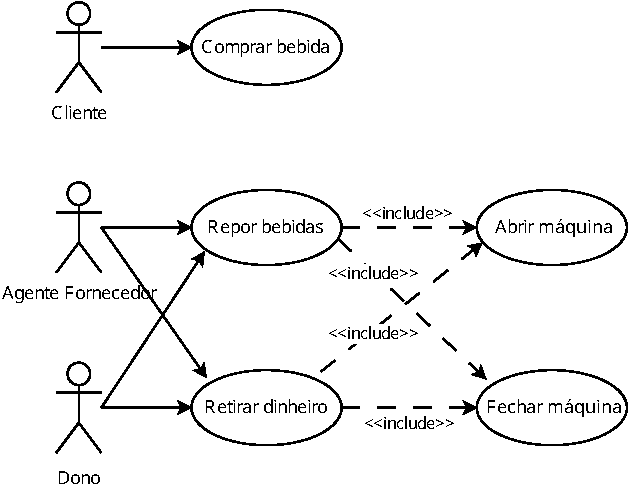
\includegraphics[width=0.58\textwidth]{imgs/UseCaseDiagramVendingMachine3.drawio.pdf}
          \caption{Possível solução apresentada de diagrama de casos de uso para o sistema de uma máquina de vendas}\label{fig:vending_machine}
      \end{figure}

      Foram ainda apresentados outros tipos de diagramas tipicamente usados no planeamento de aplicações, nomeadamente:
      \begin{itemize}
          \item \textbf{Diagrama de Estados (UML):} Descreve os diferentes estados que um objeto ou sistema pode assumir, destacando as transições entre esses estados e as ações associadas a cada um;
          
          \item \textbf{Diagrama de Sequências:} Modela a interação entre objetos num sistema em contexto temporal, exibindo a ordem das mensagens trocadas e facilitando a compreensão das dinâmicas do sistema;

          \item \textbf{Diagrama de Classes:} Um diagrama mais próximo da implementação, pois representa a estrutura do sistema orientado a objetos, mostrando classes, atributos, métodos e as relações entre as classes.
      \end{itemize}    

      Foram ainda cobertos os conceitos fundamentais de programação orientada a objetos bem como tópicos avançados como a manipulação de exceções, hierarquia, polimorfismo, e estruturas de dados. 

    \subsection{Formação de Excel}\label{subsec:excel}

      O Microsoft Excel é um programa da suíte Office 365 frequentemente utilizado para armazenar, organizar e manipular dados. É frequentemente utilizado em análise de dados ou criações de visualizações sendo muito usado no contexto da empresa, tornando a capacidade de o utilizar uma aptidão bastante favorável e procurada. 

      No entanto, esta formação acabou por tocar numa variedade de tópicos mais globais sobre boas práticas na empresa, tocando em tópicos como a forma de se apresentar e lidar com clientes, os cuidados a ter com a partilha de informação e o seu manuseamento, os cuidados a ter com a associação da marca da empresa às nossas vidas pessoais, pontualidade e mesmo a forma de resolver problemas e como a melhor contribuição para um projeto às vezes não precisa de ser técnica.

      Existem mais de 400 funções no Excel, permitindo uma interação entre dados bastante flexível, possibilitando a criação de cálculos e até gráficos e visualizações que normalmente não se associam a um programa de spreadsheets. Foram estudadas várias funções, desde a \texttt{SUM}, que simplesmente soma valores de duas células, até \texttt{VLOOKUP}, utilizada para procurar um valor específico na primeira coluna de um conjunto de dados e retornar o valor correspondente de uma coluna diferente na mesma linha. A seguinte lista não exaustiva contempla as funções estudadas durante o percurso:  

      \begin{itemize}
          \item \texttt{SUM}, \texttt{SUMIF}, \texttt{RANGE}, \texttt{CRITERIA}, \texttt{SUMIF}, \texttt{SUMIFS}, \texttt{COUNT}, \texttt{COUNTA}, \texttt{COUNTIF}, \texttt{AVERAGE}, \texttt{MAX}, \texttt{MIN}, \texttt{VLOOKUP}, \texttt{HLOOKUP}, \texttt{XLOOKUP}, \texttt{DCOUNT}, \texttt{DSUM}, \texttt{INDEX}, \texttt{ROUND}, \texttt{ROUNDUP}, \texttt{ROUNDDOWN}, \texttt{LEFT}, \texttt{RIGHT}, \texttt{MID}, \texttt{SEARCH}, \texttt{TRIM}, \texttt{IF}, \texttt{ISNA}, \texttt{MATCH}, \texttt{ISBLANK}, \texttt{ISERROR}.
      \end{itemize}    
    
    \subsection{Formação de SQL e Modelação}\label{subsec:sqlmodelacao}

      % podes ver a documentação deles para o debugger e tudo
      Dados estão em todo o tipo de aplicações, das pequenas às maiores, e estas aplicações usam bases de dados para guardar toda essa informação. A forma mais comum de guardar informação são bases de dados relacionais, constituídas por tabelas de dados que se podem relacionar entre si\cite{welcome-to-sql}. A linguagem mais amplamente usada para consultar estas bases de dados é SQL, sendo usada por uma variedade de serviços de gestão de bases de dados como Oracle, MySQL, PostgreSQL, Microsoft SQL Server\cite{sql-vs-mysql}.

      Durante a formação foram abordados todos os temas gerais da linguagem de gestão de dados, focando as seguintes características:

      \begin{itemize}
          \item \textbf{Pesquisas Básicas:} As pesquisas mais simples de SQL para obter dados das tabelas, utilizando o \texttt{SELECT}, \texttt{FROM} e \texttt{WHERE};
          
          \item \textbf{Ordenação e Agrupamento:} Usar cláusulas como \texttt{ORDER BY} e \texttt{GROUP BY} para organizar e agrupar os resultados de uma consulta SQL com base em critérios específicos;
          
          \item \textbf{Funções de Agregação:} Envolve o uso de funções como \texttt{SUM}, \texttt{AVG}, \texttt{MIN} e \texttt{MAX} para realizar cálculos em conjuntos de dados, geralmente em combinação com a cláusula \texttt{GROUP BY};
          
          \item \textbf{Junções (\textit{Joins}):} Usa-se para combinar duas ou mais tabelas usando as cláusulas \texttt{JOIN}, \texttt{INNER JOIN}, \texttt{LEFT JOIN}, \texttt{RIGHT JOIN} ou \texttt{FULL JOIN} e foram exemplificadas e visualizadas as diferenças entre cada caso;
          
          \item \textbf{Subconsultas:} Envolve o uso de consultas dentro de outras consultas, utilizando uma segunda cláusula \texttt{SELECT} na pesquisa;
          
          \item \textbf{Modificação de Dados:} Utilizou-se \texttt{INSERT}, \texttt{UPDATE}, \texttt{DELETE} e \texttt{COMMIT} para modificar e manipular os dados em tabelas específicas, ou seja, operações CRUD\footnote{CRUD (\textit{Create}, \textit{Read}, \textit{Update}, \textit{Delete}) é um acrónimo para formas de se interagir com informação guardada.}.
      \end{itemize}
    
    \subsection{Formação de Agile}\label{subsec:agilescrum}
    
      O Agile é uma abordagem de gestão de projetos e desenvolvimento com foco na flexibilidade, colaboração e satisfação do cliente. Distingue-se de outras abordagens pelo desenvolvimento iterativo, entrega incremental e capacidade de adaptação às mudanças.

      Este método diferencia-se do método tradicional Waterfall, linear com fases sequenciais, por ser iterativo. Enquanto uma abordagem Waterfall passará pelas fases de Especificação, Design, Desenvolvimento, Testes e Distribuição de forma sequencial sem avançar para um sem o último estar completo, a abordagem Agile passará por cada fase simultaneamente, entregando um resultado cada vez mais aprimorado no final de cada ciclo, como representado na Figura \ref{fig:agile-waterfall}.

      Foram transmitidos os princípios do manifesto Agile, os quais estão delineados na Tabela \ref{table:1}.

      \renewcommand{\arraystretch}{1.5}
      \begin{table}[htbp] % here top bottom page(a page just with images), ! would force it and could cause visual glitches, H is a better h that doesn't give problems by itslef (?)(https://tex.stackexchange.com/questions/132106/difference-between-h-and-h-in-float-position)
        \caption{ \href{https://agilemanifesto.org/principles.html}{Princípios do manifesto Agile}}\label{table:1}
        \source{\cite{principios-agile-manifesto}}
        \begin{tabularx}{\textwidth} { 
          >{\raggedright\arraybackslash}X 
          >{\raggedright\arraybackslash}X }
          
            %\hline
            \textbullet\ A nossa maior prioridade é satisfazer o cliente via a entrega contínua e antecipada do software. & \textbullet\ Aceitar mudanças nos requisitos, mesmo no final do desenvolvimento. Processos ágeis aproveitam  a flexibilidade das mudanças frequentes em prol vantagem competitiva do cliente. \\
            
            %\hline
            \textbullet\ Entregar software funcional frequentemente, de algumas semanas a alguns meses, com preferência no menor prazo. & \textbullet\ Pessoas de negócios e programadores devem trabalhar
            juntos diariamente ao longo do projeto. \\
            
            %\hline
            \textbullet\ Construir projetos com indivíduos motivados.
            Oferecer-lhes o ambiente e suporte necessários,
            e confiar neles para fazer um bom trabalho. & \textbullet\ O método mais eficiente e eficaz de transmitir informações para e entre uma equipa de desenvolvimento é a conversa presencial. \\
            
            %\hline
            \textbullet\ Em intervalos regulares, a equipa reflete sobre como se tornar mais eficaz, ajustando o seu comportamento. & \textbullet\ Processos ágeis promovem o desenvolvimento sustentável. Os patrocinadores, programadores e utilizadores devem ser capazes
            de manter um ritmo constante indefinidamente. \\
            
            %\hline
            \textbullet\ Atenção contínua à excelência técnica
            e bom design melhora a agilidade. & \textbullet\ Simplicidade --- a arte de maximizar a quantidade
            de trabalho não feito --- é essencial. \\
            
            %-
            
            %--

            %---

            %—

            %\textemdash
            
            %\hline
            \textbullet\ As melhores arquiteturas, requisitos e designs surgem de equipas organizadas por si mesmas. & \textbullet\ Software a funcionar é a principal medida de progresso.
        \end{tabularx}
      \end{table}

      O método ideal dependerá da do projeto, um método Waterfall é mais indicado para projetos menores e previsíveis, enquanto Agile é indicada para projetos mais avançados.

      \begin{figure}[H]
          \centering
          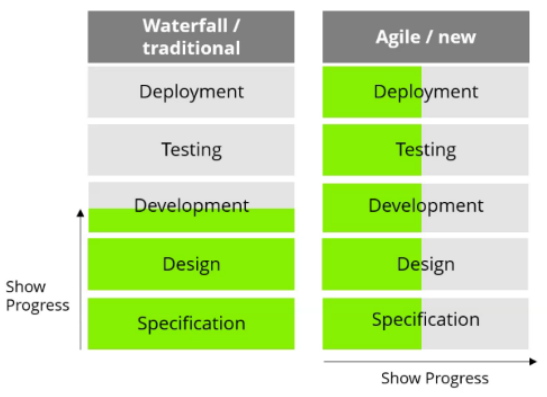
\includegraphics[scale=0.60]{imgs/agile-waterfall.png}
          \caption{Agile VS Waterfall}\label{fig:agile-waterfall}
          \source{Deloitte's Delivery Center}
      \end{figure}

    \subsubsection{Framework Scrum}\label{subsec:scrum}
    
      Scrum é um framework de Agile, especifica em detalhe como organizar o desenvolvimento, definindo papeis para as pessoas das equipas e descrevendo como aplicar o processo ágil, cuja representação gráfica apresenta-se na Figura \ref{fig:scrum}.

      \begin{figure}[H]
          \centering
          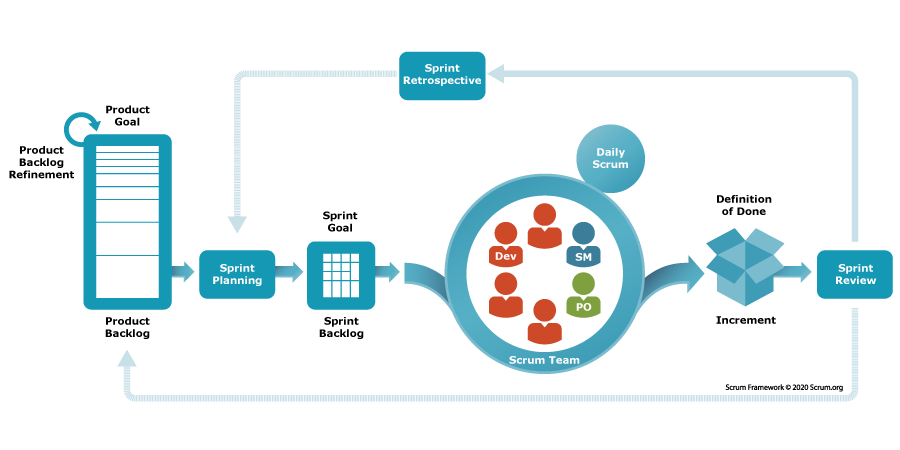
\includegraphics[scale=0.50]{imgs/scrum.png}
          \caption{\href{https://www.scrum.org/resources/what-scrum-module}{Scrum Process}}\label{fig:scrum}
          \source{\cite{scrum}}
      \end{figure}

      O Scrum requer um ambiente onde:
      \begin{itemize}
        \item Os Incrementos do trabalho são entregues em ciclos curtos de um mês ou menos, chamados \textit{sprints}. O feedback contínuo ocorre durante a \textit{sprint}, permitindo assim a inspeção e adaptação do processo e do que será entregue;
        \item A Equipa Scrum possui um \textit{Scrum Master}, um \textit{Product Owner} e Programadores, estes são responsáveis por transformar o trabalho planeado para a \textit{sprint} em algo apresentável;
        \item A Equipa Scrum e outros membros da organização, utilizadores e clientes conhecidos (\textit{stakeholders}), inspecionam os resultados da \textit{sprint} e ajustam devidamente o planeamento para a próxima.\cite{scrum}.
      \end{itemize}
    
    \subsection{Formação de OutSystems}\label{subsec:outsystems}

      OutSystems é uma plataforma \textit{low-code}\footnote{\textit{Low-code} é uma abordagem de desenvolvimento de software que minimiza a necessidade de programação manual, utilizando plataformas com interfaces gráficas e componentes reutilizáveis. Este método de desenvolvimento acelera o processo permitindo também a participação de profissionais menos experientes em programação.} para desenvolvimento, distribuição e manutenção de aplicações de forma eficiente. Com uma interface visual, como visível na Figura \ref{fig:interfaceoutsystems}, permite a criação de aplicações usando padrões bastante utilizados de forma rápida e eficaz, estando otimizado para a criação e a manutenção destas interfaces facilmente, não deixando de permitir a criação de interfaces e relações entre dados mais avançadas.

      \begin{figure}[H]
          \centering
          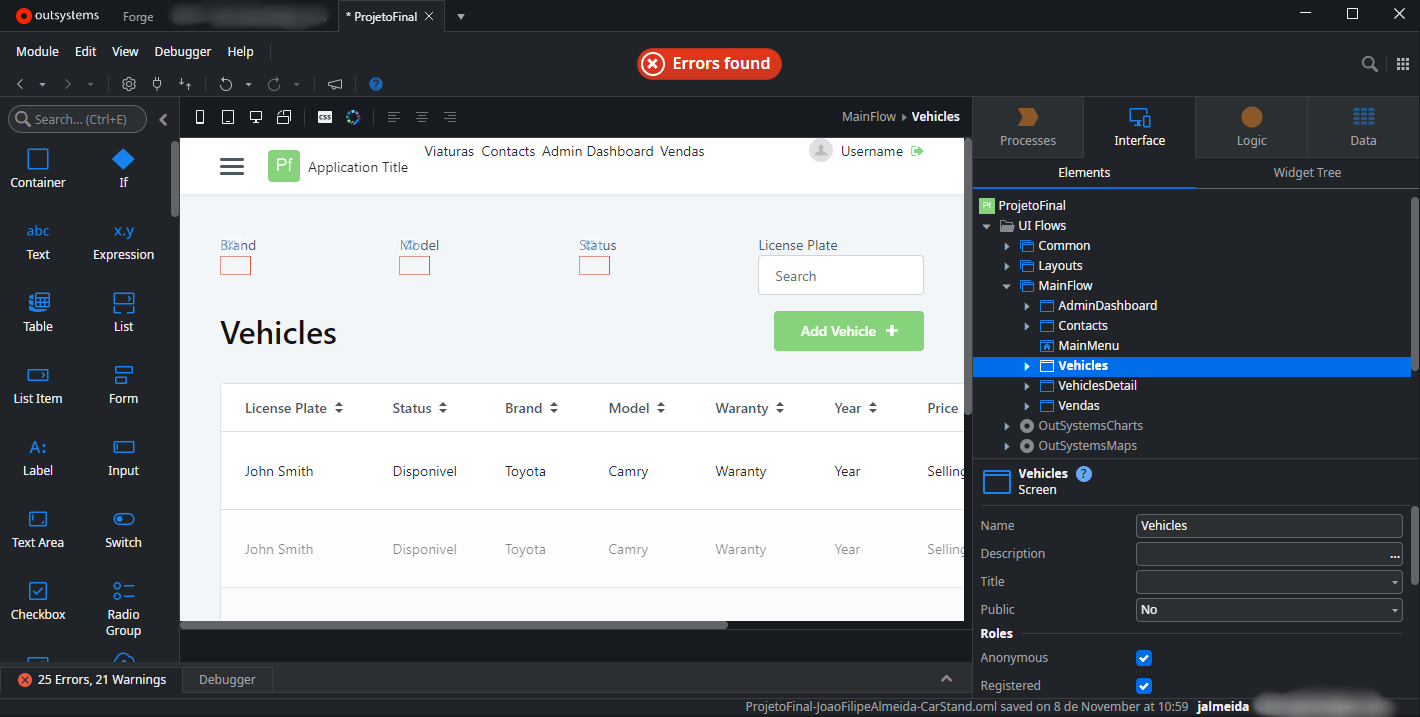
\includegraphics[width=\textwidth]{imgs/InterfaceOutSystems.png}
          \caption{Interface de OutSystems - Aplicação criada durante a formação}\label{fig:interfaceoutsystems}
          \source{Plataforma Interna da OutSystems}
      \end{figure}

      Para atingir o objetivo de ser uma plataforma visual que cubra o processo todo desde o desenvolvimento à publicação, OutSystems tem que oferecer um conjunto de ferramentas que se interliguem entre si, estas ferramentas são as seguintes:

      \begin{itemize} 
        \item \textbf{Ferramentas de Desenvolvimento:}
          \begin{itemize}
            \item \textbf{Service Studio:} Ambiente visual de desenvolvimento para aplicações Web e Mobile. Quando conectado pode publicar para o ``\textit{Platform Server}'' (servidores que compilam, publicam, gerem, executam e monitorizam aplicações.) Cada versão destas aplicações vai ser guardada na ``\textit{Platform Data Database}'';
            \item \textbf{Integration Studio:} Ambiente de desenvolvimento para criar extensões para a plataforma. Permite a criação de elementos dentro do Service Studio para interagir com recursos externos como código em C\# ou bases de dados.
          \end{itemize}
        \item \textbf{Ferramentas de Administração e Operação:}
          \begin{itemize}
            \item \textbf{Service Center:} Consola web de administração e gestão do servidor da plataforma. Inspecionar logs gerados pelo ambiente ou pelas aplicações, ou configurar definições do ambiente;
            \item \textbf{LifeTime:} Permite a gestão de todo o ciclo de vida da aplicação em vários ambientes, como, por exemplo, o ambiente de desenvolvimento, o ambiente de qualidade ou o ambiente de produção. É possível gerir as permissões de cada utilizador ou equipa, ver os ambientes e configurá-los ou a sua ordem no ciclo, analisar o desempenho das aplicações, ou efetuar \textit{deploys}\footnote{Passagem de código de um ambiente para outro de acordo com o \hyperref[fig:deployment-aggregator]{\textit{Deployment Agreaggator}}.} de código entre ambientes.
          \end{itemize}
        \item \textbf{OutSystems Forge:} Fonte de componentes para descarregar de forma a acelerar o desenvolvimento;
        \item \textbf{Comunidade:} Fóruns para troca de dicas, colocação de perguntas e obtenção de assistência\cite{outsystems-components-and-tools}.
      \end{itemize}

      Foram também explicados os conceitos mais importantes da plataforma, incluindo a aba da interface, a aba da lógica, a aba dos dados, aggregators, forms e validações, blocos e eventos, relações entre dados, \textit{roles}, Debugging. Para informação mais detalhada da plataforma, por favor refira à Secção \ref{sec:outsystems}.
    
    \subsection{Formação de Azure}\label{subsec:azure}

      A Azure é uma plataforma de computação da Microsoft, esta oferece uma panóplia de serviços Cloud para correr aplicações, servidores ou código na cloud.

      Existem três níveis distinguíveis de infraestrutura oferecidos: 
      \begin{itemize}
        \item \textbf{Infrastructure as a Service (IaaS):} IaaS é ideal quando o cliente quer manter controlo total sobre o sistema operativo e aplicações, trata-se de uma infraestrutura onde se virtualiza o hardware e o sistema operativo, deixando à responsabilidade do cliente manter o SO e as aplicações usadas atualizadas;
        \item \textbf{Platform as a Service (PaaS):} Em PaaS a plataforma de desenvolvimento e de publicação é fornecida, não é necessário gerir o sistema ou as aplicações subjacentes, mas o cliente mantém acesso ao código das aplicações que desenvolve, sendo oferecidas uma multitude de linguagens para as programar;
        \item \textbf{Software as a Service (SaaS):} Em SaaS a única responsabilidade do cliente é a gestão das contas e dos seus credenciais, SaaS refere-se ao fornecimento de aplicações já desenvolvidas para um cliente ou empresa como o Outlook ou o Office.
      \end{itemize}

      Dentro destes níveis de infraestrutura, a Microsoft disponibiliza uma variedade de serviços projetados para atender diversas necessidades, desde garantir a redundância de dados até facilitar a transferência de dados entre servidores locais, e a nuvem de Azure. Alguns destes serviços incluem:

      \begin{itemize}
          \item \textbf{Azure Blob Storage:}
          Armazenamento de objetos altamente escalável para dados não estruturados, como imagens e vídeos;
          
          \item \textbf{Azure Virtual Network:}
          Permite a criação de redes privadas na nuvem para conectar recursos Azure e estender a rede local;
          
          \item \textbf{Azure SQL Database:}
          Um serviço de bases de dados relacionais, proporcionando escalabilidade e segurança;
          
          \item \textbf{Azure ExpressRoute:}
          Estabelece conexões privadas e dedicadas à Azure, sem passar pela Internet, permitindo assim a transferência de dados rápida e seguramente;
          
          \item \textbf{Azure Backup:}
          Oferece soluções abrangentes de backup para proteger dados críticos, máquinas virtuais e aplicações;
          
          \item \textbf{Azure Logic Apps:}
          Permite a automação de fluxos de trabalho utilizando um designer visual permite a integração de serviços para criar aplicações poderosas;

          \item \textbf{Azure Cognitive Services:}
          Dezenas de serviços baseados em modelos de inteligência artificial oferecidos para integrar com as aplicações como por exemplo: Language cognitive, Speech cognitive, Vision cognitive, Decision cognitive.
      \end{itemize}

      Estes são apenas alguns exemplos dos infindáveis serviços disponíveis na plataforma Azure. Para informações mais detalhadas sobre a plataforma, por favor refira à Secção \ref{sec:plataforma-azure}.
      
    \subsection{Formação de OWASP}\label{subsec:owasp}

      A OWASP, ou \textit{Open Web Application Security Project}, é uma organização sem fins lucrativos dedicada a melhorar a segurança de software, especialmente no contexto de aplicações web. Foi fundada em 2001 e visa ajudar organizações a criar, desenvolver, obter, operar e manter aplicações que podem ser confiadas. \cite{about-the-OWASP-foundation}

      Uma das contribuições notáveis da OWASP é o \textbf{\textit{OWASP Top Ten}}. Esta é uma lista regularmente atualizada dos riscos de segurança mais críticos em aplicações web. A lista ajuda programadores, profissionais de segurança e organizações a priorizarem os seus esforços de forma a melhorar a segurança das aplicações web.
      
      As vulnerabilidades do \textit{OWASP Top ten} como especificadas em 2021 são as seguintes:

      \begin{itemize}
        \item \textbf{Controlo de Acesso Quebrado:} Problemas relacionados à má configuração ou implementação inadequada de controlos de acesso, permitindo a utilizadores não autorizados aceder a recursos protegidos;
      
        \item \textbf{Falhas Criptográficas:} Erros no uso de técnicas criptográficas, como encriptação e assinaturas digitais, que podem levar à exposição de dados sensíveis ou comprometer a segurança do sistema;
      
        \item \textbf{Injeção:} Vulnerabilidades que surgem quando dados não confiáveis são incorporados em comandos ou consultas, podendo levar à execução não autorizada de código;
      
        \item \textbf{Design Inseguro:} Riscos associados a falhas de design nas aplicações, refere-se aos riscos que não podem ser corrigidos com a implementação, salientando a importância de um planeamento adequado;
      
        \item \textbf{Configuração de Segurança:} Problemas decorrentes de configurações inadequadas ou em sintaxe errónea, especialmente em ambientes altamente configuráveis, que podem resultar em exposição não intencional de informações sensíveis;
      
        \item \textbf{Componentes Vulneráveis e Desatualizados:} Riscos relacionados ao uso de componentes (bibliotecas, frameworks) com vulnerabilidades conhecidas;
      
        \item \textbf{Falhas de Identificação e Autenticação:} Problemas de autenticação e identificação que podem permitir a utilizadores não autorizados aceder a contas protegidas ou obter privilégios indevidos;
      
        \item \textbf{Falhas de Integridade de Software e Dados:} Riscos associados a fazer suposições sobre integridade, especialmente relacionadas a atualizações de software e na utilização de extensões ou livrarias de terceiros;
      
        \item \textbf{Falhas de Registo e Monitorização de Segurança:} Desafios em garantir uma monitorização adequada e registo de eventos de segurança, o que pode afetar a visibilidade, alertas de incidentes e atividades de utilizadores;
      
        \item \textbf{Falsificação de Pedido do Lado do Servidor:} Situações em que um atacante pode induzir o servidor a fazer pedidos não autorizados em nome do utilizador\cite{OWASP-top-ten}.
      \end{itemize}

      Em suma, a OWASP é uma grande ajuda para qualquer empresa para manter um ambiente de aplicações seguras e confiáveis. A comunidade da OWASP é também bastante ativa e é ela que faz o projeto possível, contribuindo ativamente para identificar e documentar vulnerabilidades críticas.

    \subsection{Formação de MongoDB}\label{subsec:mongodb}

      O MongoDB é um sistema de gestão de bases de dados NoSQL amplamente utilizado, foi projetado para oferecer flexibilidade e escalabilidade em ambientes de desenvolvimento modernos. Ao contrário de Bases de Dados relacionais, o MongoDB adota uma abordagem baseada em documentos, armazenando dados em formato BSON (Binary JSON). A sua estrutura distribuída permite a manipulação eficiente de grandes volumes de dados, enquanto consultas mais complexas são facilitadas por índices e suporte a linguagens de consulta avançada. Além disso, o MongoDB oferece recursos de replicação para garantir alta disponibilidade e tolerância a falhas, sendo uma escolha popular para aplicações que requerem agilidade e desempenho em ambientes dinâmicos\cite{what-is-mongodb}.

      A plataforma usada para interação com estes dados através da nuvem é o Atlas, refira à Secção \ref{secsec:atlas} para mais informações sobre a plataforma.

    \subsection{Outras formações de curta duração}\label{subsec:outras-formacoes}

      De seguida apresento uma lista não exaustiva de outras formações de curta duração que muitas vezes se limitavam apenas a uma sessão ou reunião, este tipo de formações são frequentemente oferecidas sem caráter obrigatório aos empregados da empresa, e visam aprimorar as habilidades dos funcionários em diversas áreas, proporcionando-lhes uma vantagem competitiva, incentivando a versatilidade e ambientes em que os profissionais estão constantemente atualizados e no auge de sua eficiência:

    \begin{itemize}
      \item \textbf{Boas Práticas de Desenvolvimento:} Nesta formação foram abordados vários temas relacionados à criação de código legível e fácil de manter, foram abordados vários excertos analisados e simplificados colocando excertos relevantes em funções à parte, usando nomes de variáveis e funções descritivos, analisando a utilidade dos comentários, e analisando cada caso específico de forma a oferecer uma visão e capacidade geral de como fazer código profissionalmente;
      
      \item \textbf{Banca:} Focando-se no setor bancário, um setor onde se situam muitos dos clientes da companhia, foram estudados vários conceitos da área, e as formas como bancos se mantém rentáveis.
      Existem operações ativas, em que o banco se compromete a devolver o dinheiro ao cliente, como um depósito, é destas operações que o banco ganha o dinheiro que utiliza nas operações passivas, em que o cliente tem que pagar ao banco, por exemplo, um empréstimo, que terá juros;

      Foram analisados os riscos associados, incluindo: Risco de Conformidade, Risco Operacional, Risco de Sistemas de Informação, Risco de Estratégia, Risco Reputacional;
              
      \item \textbf{Seguros:} Focando-se no setor dos seguros, área também de muitos clientes da empresa, esta formação focou nos vários tipos de contratos que um individuo pode estabelecer com estas empresas e nas diferenças entre eles;
      
      \item \textbf{\textit{Getting Things Done}:} Esta formação veio a otimizar a gestão do tempo e aumentar a produtividade dos formados, proporcionando técnicas e ferramentas para a organização eficiente de tarefas pessoais e profissionais;
      
      \item \textbf{\textit{Capability Maturity Model Integration} (CMMI):} CMMI é um modelo que ajuda as organizações a otimizar a melhoria de processos e incentiva a comportamentos produtivos e eficientes que reduzem os riscos no desenvolvimento de software, produtos e serviços, definindo os seguintes níveis de maturidade: \textit{Initial}, \textit{Managed}, \textit{Defined}, \textit{Quantitatively Managed}, e \textit{Optimizing}\cite{cmmi}.

      %\item \textbf{Testes:} Abordando estratégias e práticas de teste de software, esta formação oferece conhecimentos sobre metodologias de teste, automação, e boas práticas para garantir a qualidade do software durante o ciclo de desenvolvimento.
    \end{itemize}
